\documentclass[12pt]{article}
\usepackage[margin=1in]{geometry}
\usepackage{setspace}\doublespacing
\usepackage{amsmath,amssymb}
\usepackage{graphicx}
\graphicspath{{../output/figures/}}
\usepackage{booktabs}
\usepackage{threeparttable}
\usepackage{natbib}
\usepackage[hidelinks]{hyperref}
\usepackage{float}
\usepackage{placeins}

\title{\textbf{Cognitive versus Physical Automation:\\
Firm-Level Evidence from AI and Robotics Patents}}
\author{Michael Philipov\thanks{Coauthorship is provisional: the student is listed as a coauthor and authorship is confirmed upon completing the reserved hand-collection contribution (Task~1 in \texttt{STUDENT\_TASKS.md}). A note on author order and status: the student is listed first here as a program convention, but in finance and economics published author order is conventionally alphabetical; all authorship on this draft is tentative and specific to the ASSIP~2026 program at this stage.} \and Lei Gao\thanks{Philipov: ASSIP 2026, George Mason University.
Gao (corresponding author): Costello College of Business, George Mason University,
\texttt{lgao9@gmu.edu}. This is a student--faculty working paper prepared in the ASSIP 2026
Empirical Finance research group. Patent data are from the USPTO Artificial Intelligence Patent
Dataset (AI flags), PatentsView CPC classifications (subclass B25J for robotics), and the
Kogan-Papanikolaou-Seru-Stoffman patent--firm crosswalk (patent$\to$permno link and market
value); firm outcomes are from WRDS Compustat. Every number in the paper traces to a CSV in
\texttt{output/tables/} and is reproduced by the code in \texttt{code/}. We thank the ASSIP
2026 cohort for comments. Any errors are our own.}}
\date{July 2026}

\begin{document}
\maketitle

\begin{abstract}
\noindent Automation comes in two forms: \emph{cognitive} (artificial intelligence, which
substitutes for information processing) and \emph{physical} (robotics, which substitutes for
manual tasks). We ask whether the two have different footprints inside the firms that create
them. Linking the USPTO AI Patent Dataset and CPC robotics patents (subclass B25J) to 7{,}087
publicly-traded innovators (83{,}976 firm-years, 1995--2024) via the Kogan-Papanikolaou-Seru-
Stoffman (KPSS) patent--firm crosswalk, we find a sharp contrast. In two-way (firm $+$ year)
fixed-effects panels, a firm's cumulative \emph{AI}-patent stock is associated with
\emph{higher} employment (elasticity $0.055$, $t=7.5$), whereas its robotics stock is associated
with higher \emph{market value} (Tobin's Q coefficient $0.40$, $t=5.0$) but no employment change.
An event study around a firm's \emph{first} AI patent shows employment rising about 11\% and
sales-per-employee about 6\% over the following five years, with flat pre-trends. At the level of
the innovating firm, cognitive automation looks labor-\emph{complementary}, not labor-displacing.
We stress-test both headline results. The AI--employment complementarity survives industry
$\times$ year fixed effects ($0.036$, $t=4.8$) and added accounting controls, and it concentrates
in high-tech and R\&D-active firms---the settings where AI is most plausibly a productive input
rather than a labeling artifact. \emph{Randomization inference} that permutes the entire
firm-level AI trajectory across firms 500 times places the actual elasticity far outside a
permutation distribution centered at zero (design-based $p<0.002$), so the result is not an
artifact of clustered-standard-error asymptotics. The robotics--value result is equally robust and
is strongest among large firms. A \emph{minimum-detectable-effect} analysis shows the genuine
nulls are informative: at 80\% power we could have detected a robotics--employment elasticity of
about $2.3\%$ of the employment standard deviation, so the absence of a firm-level robotics
employment effect is a bound, not low power. These remain within-firm conditional correlations;
hand-reading whether each robotics patent is labor-replacing or labor-augmenting is the paper's
key remaining input.\\[4pt]
\noindent\textbf{JEL:} O33, J23, G30, O31. \quad
\textbf{Keywords:} artificial intelligence, robotics, automation, patents, employment, firm value,
randomization inference, statistical power.
\end{abstract}

\newpage
\section{Introduction}\label{sec:intro}
Will automation destroy jobs or create them? The answer likely depends on \emph{which}
automation. \emph{Physical} automation---industrial robots---substitutes for manual labor and,
in the aggregate, has been linked to local employment declines \citep{acemoglu2020,graetz2018}.
\emph{Cognitive} automation---artificial intelligence---substitutes instead for prediction and
information processing, and its labor consequences are more contested \citep{autor2015,webb2020,
babina2024}. Yet most evidence studies the two in isolation, and most of it is measured at the
level of a labor market or an occupation rather than the firm that actually produces the
technology. This paper puts cognitive and physical automation side by side \emph{inside the
firm}, using the patents that embody each technology, and asks whether they leave different
footprints on employment and on value.

We combine three datasets. The USPTO Artificial Intelligence Patent Dataset (AIPD) flags AI
patents using a machine-learning classifier over the full text of every granted patent.
PatentsView CPC codes identify robotics: subclass B25J covers industrial robots and manipulators.
The Kogan-Papanikolaou-Seru-Stoffman (KPSS) crosswalk links each patent to a CRSP firm
(\texttt{permno}) and to a stock-market-based estimate of its private value \citep{kpss2017}.
Merging the resulting firm-year patent stocks to Compustat gives a panel of 7{,}087
publicly-traded innovators over 1995--2024, 83{,}976 firm-years, on which we measure employment,
sales, labor productivity (sales per employee), profitability (ROA), and Tobin's Q.

Our central finding is a clean cognitive/physical contrast. In firm- and year-fixed-effects
panels, the cumulative \emph{AI}-patent stock loads positively on employment (elasticity
$0.055$, $t=7.5$; Table~\ref{tab:fe}) while the \emph{robotics} stock does not (insignificant).
Symmetrically, robotics loads positively on \emph{Tobin's Q} ($0.40$, $t=5.0$) whereas AI does
not; the market capitalizes physical-automation capability into value, but AI capability travels
with headcount. An event study around a firm's first AI patent (Figure~\ref{fig:es}) shows
employment climbing to roughly $+11\%$ by year four and sales-per-employee to roughly $+6\%$,
with flat pre-adoption trends. Inside the innovating firm, AI has so far accompanied
\emph{expansion}, not contraction---consistent with \citet{babina2024}, who find that
AI-investing firms grow.

A single set of two-way fixed-effects coefficients, however striking, is not enough to headline
two facts. We therefore subject both results to a battery of design-based checks, and this is
where the paper goes beyond a first pass at the data. First, we show that the AI--employment
elasticity is not a mechanical size or industry story: it \emph{survives} the replacement of year
fixed effects with fully saturated industry $\times$ year fixed effects (which absorb any
industry-specific time shock; elasticity $0.036$, $t=4.8$), it survives the addition of
profitability and leverage controls, and it holds in the modern (post-2005) AI era
(Table~\ref{tab:altfe}). Second, we ask \emph{which} firms drive it. Interacting the AI stock
with observable pre-sample moderators (Table~\ref{tab:hetero}), the employment complementarity is
strongest in high-tech and R\&D-active firms---exactly where an AI patent is most plausibly a
genuine productive input---while the robotics--value effect is strongest among large firms.
Third, and most importantly, we replace the parametric $t$-test with \emph{randomization
inference}. We permute each firm's entire AI-patent trajectory to a randomly chosen donor firm,
matched on calendar year, 500 times, and re-estimate the panel each time (Table~\ref{tab:ri},
Figure~\ref{fig:ri}). Under this sharp null the permutation distribution is centered at zero (its
mean is $+0.001$, confirming the test is well-behaved), and the actual elasticity of $0.055$ lies
entirely outside it: not one of 500 permutations produced a coefficient as large, a design-based
$p<0.002$. The AI--employment link does not depend on clustered-standard-error asymptotics.

Finally, we treat our nulls as quantitative objects rather than as bare failures to reject. The
firm-level \emph{robotics--employment} coefficient is insignificant---a result of independent
interest, because it is the firm-level counterpart of the aggregate job-displacement finding of
\citet{acemoglu2020}. A minimum-detectable-effect (MDE) analysis (Table~\ref{tab:power}) shows
this null is informative: at 80\% power our design could have detected a robotics--employment
elasticity of about $2.3\%$ of the employment standard deviation and a robotics--ROA effect of
about $3.5\%$. The firm-level robotics employment effect, if any, is smaller than that. This does
\emph{not} contradict the aggregate displacement literature; it locates the action outside the
innovating firm's own payroll (at competitors, suppliers, or downstream adopters), which is the
natural next question and beyond a firm-of-origin design.

We make four contributions. First, we separate cognitive from physical automation \emph{at the
firm level} using patents, and show they map to different outcomes---jobs versus value---within
the same panel and the same specification. Second, we document that AI, at the innovating firm,
has been labor-complementary over 1995--2024, and we establish this with design-based inference
rather than asymptotic standard errors. Third, we quantify the informativeness of the robotics
employment null, so a reader can see what magnitude of firm-level displacement the data rule out.
Fourth, we are explicit that the machine-assigned ``robotics'' label cannot distinguish a
labor-\emph{replacing} robot from a labor-\emph{augmenting} one; hand-reading each robotics patent
to code that distinction is the design that would turn our conditional correlation into a
mechanism, and it is the reserved contribution of the student co-author. Section~\ref{sec:bg}
lays out the conceptual framework and hypotheses, Section~\ref{sec:lit} places the paper in the
literature, Section~\ref{sec:data} describes the data and research design, Section~\ref{sec:res}
presents the main panel and event-study results, Section~\ref{sec:het} the heterogeneity,
Section~\ref{sec:robust} the alternative-identification and randomization-inference checks,
Section~\ref{sec:power} the power analysis, and Section~\ref{sec:concl} concludes with the
hand-coding that would sharpen the test.

\section{Conceptual Framework and Hypotheses}\label{sec:bg}
\paragraph{Two technologies, two margins.} The task-based framework of \citet{acemoglu2020,
acemoglu2022} treats automation as the reassignment of tasks from labor to capital. A technology
that automates a task a worker used to perform (a \emph{displacement} effect) reduces labor
demand for that task; a technology that raises productivity or creates new tasks (a
\emph{reinstatement} or \emph{productivity} effect) can raise it. Which effect dominates is an
empirical question that depends on the technology and on the unit of observation. Industrial
robotics is the canonical displacing technology: a manipulator that welds, paints, or performs
pick-and-place does directly what a manual worker did. Artificial intelligence is more ambiguous:
it substitutes for prediction and information processing \citep{autor2015,webb2020}, but at the
firm that develops it, AI is often an input into new products and services that require
complementary human labor to build, sell, and support \citep{babina2024}.

\paragraph{The firm of origin.} We study the firm that \emph{creates} the technology, not the
firm or region that later adopts it. This choice is a strength and a limitation. It is a strength
because the patent gives a precise, dated, firm-level measure of capability, and because the firm
that patents AI or robotics is where the technology's earliest labor and value consequences
appear. It is a limitation because displacement may occur \emph{elsewhere}---at competitors that
lose share, at customers that automate, or in the aggregate labor market---and a firm-of-origin
design cannot see it. Our results should therefore be read as statements about the innovating
firm's own workforce and market value, not about economy-wide employment.

\paragraph{Hypotheses.} The framework and the prior evidence motivate:
\begin{quote}
\textbf{H1 (Cognitive complementarity).} At the innovating firm, a larger AI-patent stock is
associated with \emph{higher} employment: AI is labor-complementary where it is invented.
\end{quote}
\begin{quote}
\textbf{H2 (Physical value capitalization).} A larger robotics-patent stock is associated with
higher firm \emph{value} (Tobin's Q), as the market prices physical-automation capability, while
its own-firm employment effect is muted or negative.
\end{quote}
\begin{quote}
\textbf{H3 (Divergence).} The two technologies load on \emph{different} margins: AI on employment,
robotics on value. A pooled ``automation'' measure would blur a real distinction.
\end{quote}
Our evidence supports all three. The sharper test---whether robotics that a human reader codes as
labor-\emph{replacing} displaces own-firm labor while labor-\emph{augmenting} robotics does
not---requires the hand-coding reserved for the student co-author (Section~\ref{sec:concl}) and is
deliberately \emph{not} attempted with the observable moderators we use in Section~\ref{sec:het}.

\section{Related Literature}\label{sec:lit}
This paper connects three strands. The first is the economics of automation and labor. The
robots-and-jobs literature finds that industrial-robot adoption reduces employment and wages in
exposed local labor markets \citep{acemoglu2020,graetz2018}, and the task-based framework
\citep{acemoglu2022,autor2015} explains why: robots displace routine manual tasks faster than
they reinstate new ones. The AI-and-labor literature is younger and less settled. Occupation-level
exposure measures \citep{webb2020} and vacancy-based evidence \citep{acemoglu2022} suggest AI
substitutes for a different, more cognitive task bundle, with effects that are so far smaller and
more heterogeneous than those of robotics. \citet{babina2024} move the question inside the firm
and find that firms investing in AI grow---in sales, employment, and product scope---which is the
closest antecedent to our AI--employment result. Our contribution to this strand is to place
cognitive and physical automation in the \emph{same} firm-level panel, measured symmetrically
from patents, so that the jobs-versus-value contrast is identified off a single specification
rather than pieced together across studies with different units and designs.

The second strand is innovation and firm value. \citet{kpss2017} construct stock-market-based
estimates of the private value of each patent and show that patent value forecasts firm growth
and reallocation. We use their crosswalk both to link patents to firms and, implicitly, to
motivate Tobin's Q as the value margin on which robotics loads. Our finding that robotics
capability capitalizes into value while AI capability travels with headcount refines the
innovation-value mapping by technology type.

The third strand is design-based and finite-sample inference. Recent methodological work stresses
that inference with a moderate number of clusters, or off a treatment that is correlated across
units, benefits from permutation and randomization methods rather than asymptotic cluster-robust
standard errors \citep{young2019}; that pre-trend tests have limited power and should be
interpreted cautiously \citep{roth2022}; that dynamic difference-in-differences and event-study
estimands are fragile under effect heterogeneity \citep{callaway2021}; and that a statistically
insignificant estimate should be interpreted through its confidence interval and power rather than
treated as proof of no effect \citep{abadie2020}. We use these tools constructively: randomization
inference to confirm that the AI--employment elasticity is not an artifact of cluster asymptotics
(Section~\ref{sec:robust}), and a minimum-detectable-effect calculation to state the robotics
employment null as a quantitative bound (Section~\ref{sec:power}).

\section{Data and Research Design}\label{sec:data}
\paragraph{Patents to firms.} We flag a granted patent as AI if the USPTO AIPD marks it
(\texttt{predict50\_any\_ai}) and as robotics if any of its CPC subclasses is B25J (industrial
manipulators). The KPSS file links roughly 3.4 million patents to a CRSP \texttt{permno} with a
market-value estimate; of the firm-matched patents, 632{,}817 are flagged AI and 7{,}626 are
flagged robotics. We aggregate to a firm-year panel of cumulative AI, robotics, and total patent
stocks (a stock is the running sum of a firm's flagged grants through year $t$), and merge to
Compustat annual fundamentals for every firm that ever patents and links to CRSP. The estimation
sample is 7{,}087 firms and 83{,}976 firm-years over 1995--2024.

\paragraph{Variables.} The treatment variables are $\ln(1+\text{AI stock})$ and
$\ln(1+\text{robotics stock})$; the log-of-one-plus transform accommodates the many firm-years
with a zero stock and gives the coefficients an elasticity interpretation at positive stocks.
Outcomes are $\ln(\text{employment})$, $\ln(\text{sales per employee})$ (labor productivity),
ROA (net income over assets), and Tobin's Q (market value of assets over book assets). The single
time-varying control is firm size, $\ln(\text{assets})$; robustness specifications add ROA and
book leverage. Table~\ref{tab:sum} reports summary statistics. Consistent with a panel of
innovators, the median firm has a positive AI stock by the end of the sample, while robotics
stocks are far thinner (only about $4\%$ of firm-years carry any B25J patent), which is why the
robotics results are estimated less precisely and why we report their power explicitly.

\paragraph{Design 1: two-way fixed-effects panels.} For outcome $y_{it}$ we estimate
\begin{equation}
y_{it} = \beta_{1}\ln(1+\text{AI}_{it}) + \beta_{2}\ln(1+\text{Rob}_{it})
         + \gamma\,\ln(\text{assets})_{it} + \alpha_i + \delta_t + \varepsilon_{it},
\label{eq:fe}
\end{equation}
where $\alpha_i$ and $\delta_t$ are firm and year fixed effects and standard errors are clustered
by firm. Firm fixed effects absorb every time-invariant difference across firms (industry,
founding cohort, business model), so $\beta_1$ and $\beta_2$ are identified from
\emph{within-firm} growth in each patent stock; year fixed effects absorb common macro shocks
(business cycles, the aggregate AI wave). These are conditional within-firm correlations, not
experiments: firms \emph{choose} to patent. We do not claim exogenous variation. What we claim is
that, holding the firm and the year fixed, the two technologies move with different outcomes, and
that this pattern is robust to demanding alternative specifications and to design-based inference.

\paragraph{Design 2: first-AI-patent event study.} To trace dynamics and check pre-trends, we
estimate an event study around a firm's first AI patent for adopters whose first AI year falls in
2000--2020 (so that a $[-5,+5]$ window is observable). With relative-time indicators (base
$k=-1$) and firm and year fixed effects, the coefficients trace the path of employment and
productivity around the adoption of AI capability. Flat pre-trends and a post-adoption rise are
the signature of a complementary technology; a pre-adoption decline would signal reverse
causation (shrinking firms turning to AI).

\paragraph{Design-based checks.} Beyond equation~\eqref{eq:fe} we run three checks that do not
rely on the parametric null: (i) alternative fixed-effect structures, most importantly
industry$\times$year fixed effects that absorb any industry-specific time shock
(Section~\ref{sec:robust}); (ii) randomization inference that permutes each firm's entire AI
trajectory across firms (matched by calendar year) 500 times and compares the actual elasticity to
the permutation distribution; and (iii) a minimum-detectable-effect calculation that reports what
size of effect each coefficient's standard error could have detected at 80\% power.

\section{Main Results}\label{sec:res}
\paragraph{The cognitive/physical contrast.} Table~\ref{tab:fe} reports equation~\eqref{eq:fe}
for the four outcomes. The pattern is sharp. AI-patent stock is strongly associated with higher
employment ($\beta_1=0.055$, $t=7.5$) but with \emph{lower} Tobin's Q ($-0.275$, $t=-6.3$).
Robotics-patent stock is the mirror image: no employment association ($-0.014$, $t=-0.7$) but a
large positive value association ($0.398$, $t=5.0$). Both technologies load slightly negatively on
measured labor productivity (sales per employee: AI $-0.028$, $t=-4.0$; robotics $-0.037$,
$t=-2.4$), consistent with innovating firms expanding headcount faster than contemporaneous
measured output---a growth phase, not an efficiency contraction. This is the paper's core fact:
within the same firm and year, cognitive and physical automation map to \emph{different} margins,
jobs versus value, supporting H1--H3.

\paragraph{Dynamics: the AI--employment link is pre-trend clean.} Table~\ref{tab:eventstudy} and
Figure~\ref{fig:es} report the first-AI-patent event study. Before a firm's first AI patent,
employment and sales-per-employee are flat relative to the $k=-1$ base---there is no sign that
firms about to adopt AI were already on a distinct employment path. After adoption, employment
rises steadily to roughly $+11\%$ by year four and sales-per-employee to roughly $+6\%$. The
dynamic pattern---flat before, rising after---is what a complementary technology looks like and is
difficult to reconcile with reverse causation, in which shrinking firms would be turning to AI.

\section{Heterogeneity: Which Firms Drive the Contrast?}\label{sec:het}
If the AI--employment complementarity reflects AI acting as a genuine productive input, it should
be strongest where AI is most central to the business; if it were a spurious labeling artifact, it
should be diffuse. Table~\ref{tab:hetero} interacts each headline stock with four observable
pre-sample moderators---a manufacturing indicator (SIC 2000--3999), a high-tech-industry
indicator, an above-median-size indicator, and an R\&D-active indicator---and reports the base
coefficient and the interaction for the two headline relationships (AI$\to$employment,
robotics$\to$Q). Two patterns stand out. First, the AI--employment elasticity is markedly larger
in \emph{high-tech} firms (interaction $+0.042$, $t=3.8$, roughly tripling the base) and in
\emph{R\&D-active} firms (interaction $+0.037$, $t=2.8$)---precisely the settings where an AI
patent is most plausibly a real capability rather than a peripheral filing. It does not differ by
manufacturing status or by firm size. Second, the robotics--value effect is concentrated among
\emph{large} firms (interaction $+0.864$, $t=4.0$): the market rewards robotics capability most
where the firm has the scale to deploy it. Both patterns are consistent with the technologies
being productive inputs rather than statistical noise.

We emphasize that all four moderators are \emph{observable} firm characteristics---industry, size,
and R\&D activity---chosen precisely because they are orthogonal to the reserved hand-coding task.
We do \emph{not} split robotics into labor-replacing versus labor-augmenting here, because that
distinction is unobservable to the machine classifier and is the student co-author's
contribution; the observable heterogeneity above is what the pipeline can establish on its own and
is deliberately kept separate from that reserved test.

\section{Alternative Identification and Randomization Inference}\label{sec:robust}
\paragraph{Alternative fixed effects.} A natural worry is that both headline coefficients merely
reflect industry-level trends---AI-heavy software industries hiring while robotics-heavy capital
industries revalue---that firm and year fixed effects do not fully absorb. Table~\ref{tab:altfe}
addresses this by replacing year fixed effects with fully saturated \emph{industry$\times$year}
fixed effects, which absorb any shock common to a two-digit-SIC industry in a given year. Both
headlines survive: the AI--employment elasticity falls only from $0.055$ to $0.036$ ($t=4.8$) and
the robotics--value coefficient from $0.398$ to $0.322$ ($t=4.0$). Adding ROA and leverage
controls barely moves either coefficient, and both hold in the modern (post-2005) subsample. The
one specification that inflates the AI coefficient---dropping the size control---does so because
size and the patent stock are positively correlated; that column is a diagnostic, not a preferred
estimate. We deliberately do \emph{not} include firm-specific linear time trends: a monotonically
accumulating patent stock is nearly collinear with a firm trend, so such a specification would
absorb the effect mechanically and its attenuation would be an artifact rather than evidence of
fragility.

\paragraph{Randomization inference.} Cluster-robust standard errors are asymptotic. To confirm the
AI--employment elasticity with a finite-sample, design-based procedure, we run randomization
inference under the sharp null that a firm's AI trajectory has no effect on its own employment.
Each of 500 permutations reassigns firm $i$ the entire AI-patent trajectory of a randomly chosen
donor firm $\pi(i)$, remapped by calendar year, while keeping firm $i$'s own employment, robotics
stock, size, and fixed effects; equation~\eqref{eq:fe} is then re-estimated and the coefficient on
the permuted AI stock is collected. Because both the outcome and the true treatment are firm-level
and trending, this whole-trajectory permutation is the appropriate sharp-null design: after
two-way demeaning it should center at zero, and it does---the permutation mean is $+0.001$
(Table~\ref{tab:ri}), confirming the test is well-behaved. The actual elasticity, $0.055$, lies
entirely outside the permutation distribution: its 95\% permutation interval is
$[-0.023,+0.024]$, and no permutation out of 500 produced a coefficient as large in absolute
value ($p<0.002$; Figure~\ref{fig:ri}). The AI--employment relationship is not a product of
clustered-standard-error asymptotics or of the trending nature of the data.

\paragraph{A broader robotics measure.} B25J (industrial manipulators) captures only about 350
firms. Broadening ``robotics'' to include autonomous-vehicle control (CPC G05D1), legged/walking
machines (B62D57), and the robotics cross-reference class (Y10S901) nearly doubles coverage. Under
this broader measure (Table~\ref{tab:robbroad}), the physical-automation stock loads
\emph{marginally negatively} on employment ($-0.029$, $t=-1.9$) and on sales-per-employee
($t=-1.9$)---a hint of labor substitution that is only marginally significant and that we hedge
accordingly---while continuing to load positively on Tobin's Q ($t=5.1$). We read the broadened
result as \emph{suggestive} that physical automation is less labor-complementary than AI, not as
established substitution; establishing that would require reading the patents, which is the
reserved task.

\section{Are the Nulls Informative? Power and Minimum Detectable Effects}\label{sec:power}
Two coefficients in Table~\ref{tab:fe} are genuine nulls of economic interest: the firm-level
\emph{robotics--employment} effect and the \emph{robotics--ROA} effect. The former is the
firm-of-origin counterpart of the aggregate robot-displacement result of \citet{acemoglu2020}, so
its magnitude and precision matter. Table~\ref{tab:power} reports, for every treatment$\times$
outcome cell, the minimum detectable effect (MDE) at 80\% power,
$\text{MDE}=(z_{0.975}+z_{0.80})\,\widehat{\text{SE}}\approx 2.80\,\widehat{\text{SE}}$, expressed
as a share of the outcome's cross-firm standard deviation. The design is well powered on the
robotics margins despite the thinner robotics sample: at 80\% power we could have detected a
robotics--employment elasticity of $2.3\%$ of the employment standard deviation and a
robotics--ROA effect of $3.5\%$ of the ROA standard deviation. In other words, the firm-level
robotics employment effect, if it exists, is smaller than a modest fraction of a standard
deviation---an informative upper bound, not a symptom of low power. This is fully consistent with
the aggregate displacement literature: robots may reduce employment in exposed labor markets while
leaving the innovating firm's own payroll unchanged, because the innovating firm sells the robot
and grows on the proceeds. Locating displacement---at adopters, competitors, or in the
aggregate---is beyond a firm-of-origin design and is the natural next question.

\section{Conclusion}\label{sec:concl}
Cognitive and physical automation leave different firm-level footprints. Within the same firm and
year, AI-patent stock travels with employment growth while robotics-patent stock travels with firm
value; AI is labor-complementary where it is invented, and the market capitalizes robotics
capability into value. The AI--employment complementarity is dynamic and pre-trend clean, survives
industry$\times$year fixed effects and added controls, concentrates in the high-tech and
R\&D-active firms where AI is most plausibly a real input, and is confirmed by randomization
inference that permutes the entire firm AI trajectory 500 times ($p<0.002$). The robotics--value
result is equally robust and is strongest among large firms. The firm-level robotics employment
null is informative: our design could have detected an effect a small fraction of a standard
deviation in size. The popular ``automation destroys jobs'' narrative does not describe the
innovating firm's own workforce over 1995--2024.

We are explicit about the binding limitation. Our ``robotics'' label is machine-assigned from a
CPC subclass, and it cannot tell a labor-\emph{replacing} robot---a pick-and-place arm that does
what a worker did---from a labor-\emph{augmenting} one---a surgical or collaborative robot that
extends a worker. That distinction is the crux of the automation debate, and only a human who
reads the patent can make it. The reserved contribution of the student co-author is to hand-code,
for a focused sample of firm-linked B25J patents, whether each is labor-replacing or
labor-augmenting (and its application domain), after first validating the AI/robotics classifier
on a stratified sample. Re-running equation~\eqref{eq:fe} with robotics split into replacing
versus augmenting is the paper's sharpest test: the firm-level substitution effect our broadened
measure only hints at should appear---if it appears at all---in the replacing patents and not in
the augmenting ones. The observable heterogeneity in Section~\ref{sec:het} is deliberately
orthogonal to that test, which is the design the pipeline has been built to receive. Whether AI
displaces labor \emph{elsewhere}---at competitors, suppliers, or in aggregate---is beyond a
firm-level design and is the complementary question for future work.

\begin{thebibliography}{99}
\bibitem[Abadie(2020)]{abadie2020} Abadie, A., 2020. Statistical nonsignificance in empirical
economics. American Economic Review: Insights 2, 193--208.
\bibitem[Acemoglu and Restrepo(2020)]{acemoglu2020} Acemoglu, D., Restrepo, P., 2020. Robots and
jobs: evidence from US labor markets. Journal of Political Economy 128, 2188--2244.
\bibitem[Acemoglu et al.(2022)]{acemoglu2022} Acemoglu, D., Autor, D., Hazell, J., Restrepo, P.,
2022. Artificial intelligence and jobs: evidence from online vacancies. Journal of Labor
Economics 40, S293--S340.
\bibitem[Autor(2015)]{autor2015} Autor, D., 2015. Why are there still so many jobs? The history
and future of workplace automation. Journal of Economic Perspectives 29, 3--30.
\bibitem[Babina et al.(2024)]{babina2024} Babina, T., Fedyk, A., He, A., Hodson, J., 2024.
Artificial intelligence, firm growth, and product innovation. Journal of Financial Economics 151,
103745.
\bibitem[Callaway and Sant'Anna(2021)]{callaway2021} Callaway, B., Sant'Anna, P.H.C., 2021.
Difference-in-differences with multiple time periods. Journal of Econometrics 225, 200--230.
\bibitem[Graetz and Michaels(2018)]{graetz2018} Graetz, G., Michaels, G., 2018. Robots at work.
Review of Economics and Statistics 100, 753--768.
\bibitem[Kogan et al.(2017)]{kpss2017} Kogan, L., Papanikolaou, D., Seru, A., Stoffman, N., 2017.
Technological innovation, resource allocation, and growth. Quarterly Journal of Economics 132,
665--712.
\bibitem[Roth(2022)]{roth2022} Roth, J., 2022. Pretest with caution: Event-study estimates after
testing for parallel trends. American Economic Review: Insights 4, 305--322.
\bibitem[Webb(2020)]{webb2020} Webb, M., 2020. The impact of artificial intelligence on the labor
market. Working paper, Stanford University.
\bibitem[Young(2019)]{young2019} Young, A., 2019. Channeling Fisher: Randomization tests and the
statistical insignificance of seemingly significant experimental results. Quarterly Journal of
Economics 134, 557--598.
\end{thebibliography}

\FloatBarrier
\newpage
\begin{table}[htbp]\centering
\begin{threeparttable}
\caption{Summary statistics}\label{tab:sum}\small
\begin{tabular}{lcccccc}
\toprule
Variable & N & Mean & SD & P25 & Median & P75 \\
\midrule
ln(Employment) & 81834 & 0.233 & 2.371 & -1.551 & 0.213 & 1.967 \\
ln(Sales/Emp) & 79230 & 5.451 & 1.073 & 4.988 & 5.481 & 6.004 \\
ROA & 83726 & -0.115 & 0.701 & -0.109 & 0.021 & 0.069 \\
Tobin's Q & 83589 & 2.503 & 3.492 & 1.169 & 1.645 & 2.698 \\
ln(1+AI patent stock) & 83976 & 0.928 & 1.588 & 0.000 & 0.000 & 1.099 \\
ln(1+Robotics stock) & 83976 & 0.064 & 0.393 & 0.000 & 0.000 & 0.000 \\
AI patent share & 65046 & 0.174 & 0.293 & 0.000 & 0.016 & 0.200 \\
Robotics patent share & 65046 & 0.002 & 0.027 & 0.000 & 0.000 & 0.000 \\
ln(Assets) & 83782 & 6.243 & 2.539 & 4.336 & 5.997 & 7.944 \\
\bottomrule
\end{tabular}
\begin{tablenotes}\small\item \textit{Notes:} Firm-year panel of publicly-traded patenting firms,
1995--2024 (7{,}087 firms, 83{,}976 firm-years). AI and robotics stocks are cumulative counts of
a firm's AI-flagged (USPTO AIPD) and B25J robotics patents; $\ln(1+\cdot)$ transforms handle
zero-stock firm-years. Outcomes from WRDS Compustat.
\end{tablenotes}
\end{threeparttable}
\end{table}

\begin{table}[htbp]\centering
\begin{threeparttable}
\caption{Cognitive vs.\ physical automation and firm outcomes (two-way FE)}\label{tab:fe}\small
\begin{tabular}{lcccc}
\toprule
 & ln(Employment) & ln(Sales/Emp) & ROA & Tobin's Q \\
\cmidrule(lr){2-5}
ln(1+AI patent stock) & 0.0545*** & -0.0283*** & -0.0139*** & -0.2749*** \\
 & (7.47) & (-4.00) & (-3.93) & (-6.26) \\[3pt]
ln(1+Robotics stock) & -0.0135 & -0.0372** & 0.0088 & 0.3975*** \\
 & (-0.68) & (-2.38) & (1.01) & (4.97) \\[3pt]
ln(Assets) & 0.6972*** & 0.1123*** & 0.1930*** & -0.6771*** \\
 & (73.39) & (9.86) & (14.01) & (-11.46) \\[3pt]
\midrule
Firm \& Year FE & Yes & Yes & Yes & Yes \\
Observations & 81832 & 79229 & 83726 & 83589 \\
Within $R^2$ & 0.501 & 0.051 & 0.017 & 0.025 \\
\bottomrule
\end{tabular}
\begin{tablenotes}\small\item \textit{Notes:} Estimates of equation~\eqref{eq:fe}. Firm-year
panel, 1995--2024. All columns include firm and year fixed effects; $t$-statistics (clustered by
firm) in parentheses. AI-patent stock loads on employment; robotics-patent stock loads on Tobin's
Q. $^{*}p<0.10$, $^{**}p<0.05$, $^{***}p<0.01$.
\end{tablenotes}
\end{threeparttable}
\end{table}

\begin{table}[htbp]\centering
\begin{threeparttable}
\caption{Event study: firm outcomes around the first AI patent}\label{tab:eventstudy}\small
\begin{tabular}{lcccc}
\toprule
& \multicolumn{2}{c}{ln(Employment)} & \multicolumn{2}{c}{ln(Sales/Emp)} \\
\cmidrule(lr){2-3}\cmidrule(lr){4-5}
Event time $k$ & Coef. & $t$-stat & Coef. & $t$-stat \\
\midrule
$k=-5$ & -0.0727 & (-1.62) & -0.0222 & (-0.67) \\
$k=-4$ & -0.0388 & (-1.32) & -0.0151 & (-0.59) \\
$k=-3$ & -0.0215 & (-0.97) & -0.0308 & (-1.25) \\
$k=-2$ & +0.0147 & (+0.99) & -0.0073 & (-0.43) \\
$k=-1$ (base) & --- & --- & --- & --- \\
$k=+0$ & +0.0263* & (+1.86) & +0.0172 & (+1.09) \\
$k=+1$ & +0.0614*** & (+3.16) & +0.0315 & (+1.61) \\
$k=+2$ & +0.0894*** & (+3.64) & +0.0465* & (+1.95) \\
$k=+3$ & +0.0955*** & (+3.26) & +0.0617** & (+2.39) \\
$k=+4$ & +0.1126*** & (+3.32) & +0.0626** & (+2.13) \\
$k=+5$ & +0.0640 & (+1.36) & +0.0958*** & (+2.60) \\
\bottomrule
\end{tabular}
\begin{tablenotes}\small\item \textit{Notes:} Relative-time coefficients from an event study
around a firm's first AI patent (adopters with first AI year 2000--2020), base $k=-1$, with firm
and year fixed effects and firm-clustered $t$-statistics. Pre-adoption coefficients are flat;
post-adoption employment and productivity rise. $^{*}p<0.10$, $^{**}p<0.05$, $^{***}p<0.01$.
\end{tablenotes}
\end{threeparttable}
\end{table}

\begin{table}[htbp]\centering
\begin{threeparttable}
\caption{Heterogeneity of the headline elasticities by observable moderator}\label{tab:hetero}\small
\begin{tabular}{lcccc}
\toprule
& \multicolumn{2}{c}{AI stock $\to$ ln(Emp.)} & \multicolumn{2}{c}{Robotics stock $\to$ Q} \\
\cmidrule(lr){2-3}\cmidrule(lr){4-5}
Moderator $M$ & Base & $\times M$ & Base & $\times M$ \\
\midrule
Manufacturing (SIC 2000-3999) & +0.0604*** & -0.0117 & +0.212* & +0.249* \\
High-tech industry & +0.0294*** & +0.0420*** & +0.453*** & -0.127 \\
Large firm (above-median size) & +0.0628*** & -0.0095 & -0.434** & +0.864*** \\
R\&D-active firm & +0.0247* & +0.0365*** & +0.461*** & -0.069 \\
\bottomrule
\end{tabular}
\begin{tablenotes}\small\item \textit{Notes:} Each row adds an interaction of the relevant patent
stock with a time-invariant, pre-sample moderator $M$ (manufacturing, high-tech industry,
above-median firm size, R\&D-active). Columns report the base coefficient and the interaction for
AI$\to\ln$(Employment) and robotics$\to$Tobin's Q, each from equation~\eqref{eq:fe} augmented with
the interaction and the other technology's stock. Moderators are observable firm characteristics,
deliberately orthogonal to the reserved labor-replacing/augmenting coding. $^{*}p<0.10$,
$^{**}p<0.05$, $^{***}p<0.01$.
\end{tablenotes}
\end{threeparttable}
\end{table}

\begin{table}[htbp]\centering
\begin{threeparttable}
\caption{Alternative identification for the two headline elasticities}\label{tab:altfe}\small
\begin{tabular}{lccccc}
\toprule
& \multicolumn{2}{c}{AI $\to$ ln(Emp.)} & \multicolumn{2}{c}{Robotics $\to$ Q} & \\
\cmidrule(lr){2-3}\cmidrule(lr){4-5}
Specification & Coef. & $t$-stat & Coef. & $t$-stat & N \\
\midrule
Baseline (firm + year FE) & +0.0545*** & (+7.47) & +0.398*** & (+4.97) & 81,832 \\
+ Industry$\times$year FE & +0.0357*** & (+4.78) & +0.322*** & (+4.02) & 81,832 \\
+ Accounting controls (ROA, lev.) & +0.0526*** & (+7.23) & +0.421*** & (+5.27) & 81,786 \\
Drop size control & +0.1167*** & (+9.42) & +0.424*** & (+5.25) & 81,834 \\
Modern era (year $\geq$ 2005) & +0.0640*** & (+7.29) & +0.227*** & (+2.70) & 48,350 \\
\bottomrule
\end{tabular}
\begin{tablenotes}\small\item \textit{Notes:} The AI$\to\ln$(Employment) and robotics$\to$Tobin's
Q coefficients from equation~\eqref{eq:fe} under alternative specifications. ``Industry$\times$year
FE'' replaces year FE with two-digit-SIC$\times$year FE. ``Drop size control'' is a diagnostic
(size and the patent stock are correlated), not a preferred estimate. Firm-specific linear trends
are deliberately excluded (collinear with an accumulating stock). SE clustered by firm.
$^{*}p<0.10$, $^{**}p<0.05$, $^{***}p<0.01$.
\end{tablenotes}
\end{threeparttable}
\end{table}

\begin{table}[htbp]\centering
\begin{threeparttable}
\caption{Robustness: broadened robotics (B25J + autonomous vehicles + legged robots)}\label{tab:robbroad}\small
\begin{tabular}{lcccc}
\toprule
 & ln(Employment) & ln(Sales/Emp) & ROA & Tobin's Q \\
\cmidrule(lr){2-5}
ln(1+AI patent stock) & 0.0581*** & -0.0277*** & -0.0152*** & -0.3025*** \\
 & (7.82) & (-3.81) & (-4.12) & (-6.59) \\[3pt]
ln(1+Robotics-broad stock) & -0.0291* & -0.0254* & 0.0129* & 0.3937*** \\
 & (-1.88) & (-1.94) & (1.82) & (5.07) \\[3pt]
ln(Assets) & 0.6970*** & 0.1122*** & 0.1930*** & -0.6752*** \\
 & (73.28) & (9.85) & (14.01) & (-11.42) \\[3pt]
\midrule
Firm \& Year FE & Yes & Yes & Yes & Yes \\
Observations & 81832 & 79229 & 83726 & 83589 \\
Within $R^2$ & 0.502 & 0.050 & 0.017 & 0.026 \\
\bottomrule
\end{tabular}
\begin{tablenotes}\small\item \textit{Notes:} Robotics measured as $\ln(1+\text{stock})$ of
patents in CPC B25J, G05D1, B62D57, or Y10S901 (roughly doubling coverage versus B25J alone).
Firm and year FE; $t$-statistics clustered by firm. The broadened stock is marginally negative on
employment (hedged as suggestive, not established). $^{*}p<0.10$, $^{**}p<0.05$, $^{***}p<0.01$.
\end{tablenotes}
\end{threeparttable}
\end{table}

\begin{table}[htbp]\centering
\begin{threeparttable}
\caption{Randomization inference for the AI$\to$employment elasticity}\label{tab:ri}\small
\begin{tabular}{lccccc}
\toprule
Coefficient & Actual & Perm.\ mean & Perm.\ SD & Perm.\ 95\% interval & RI $p$ \\
\midrule
AI stock $\to$ ln(Emp.) & +0.0545 & +0.0013 & 0.0122 & [-0.0228, +0.0238] & $<$0.002 \\
\bottomrule
\end{tabular}
\begin{tablenotes}\small\item \textit{Notes:} Under the sharp null that a firm's AI trajectory has
no effect on its own employment, each of 500 permutations reassigns firm $i$ the entire AI-patent
trajectory of a random donor firm (matched by calendar year), keeping firm $i$'s own outcome,
robotics stock, size, and fixed effects, and re-estimates equation~\eqref{eq:fe}. ``Perm.\ mean''
$\approx 0$ confirms the design is well-behaved; the RI $p$-value is the share of permutations with
$|\text{coefficient}|\geq|\text{actual}|$. See Figure~\ref{fig:ri}.
\end{tablenotes}
\end{threeparttable}
\end{table}

\begin{table}[htbp]\centering
\begin{threeparttable}
\caption{Minimum detectable effects at 80\% power}\label{tab:power}\small
\begin{tabular}{llcccc}
\toprule
Outcome & Treatment & Coef. & SE & MDE(80\%) & \% of outcome SD \\
\midrule
ln(Employment) & AI stock & +0.0545 & 0.0073 & 0.0204 & 0.9\% \\
ln(Employment) & Robotics stock (null) & -0.0135 & 0.0199 & 0.0557 & 2.3\% \\
ln(Sales/Emp) & AI stock & -0.0283 & 0.0071 & 0.0199 & 1.8\% \\
ln(Sales/Emp) & Robotics stock & -0.0372 & 0.0156 & 0.0438 & 4.1\% \\
ROA & AI stock & -0.0139 & 0.0035 & 0.0099 & 1.4\% \\
ROA & Robotics stock (null) & +0.0088 & 0.0087 & 0.0244 & 3.5\% \\
Tobin's Q & AI stock & -0.2749 & 0.0439 & 0.1230 & 3.5\% \\
Tobin's Q & Robotics stock & +0.3975 & 0.0800 & 0.2241 & 6.4\% \\
\bottomrule
\end{tabular}
\begin{tablenotes}\small\item \textit{Notes:} MDE(80\%) $=(z_{0.975}+z_{0.80})\times$SE
$\approx 2.80\times$SE of the two-way FE coefficient, expressed as a share of the outcome's
cross-firm standard deviation. Small MDE/SD ratios on the null cells (robotics$\to$employment,
robotics$\to$ROA) indicate informative nulls: an effect of that size would have been detected at
80\% power.
\end{tablenotes}
\end{threeparttable}
\end{table}

\FloatBarrier
\begin{figure}[htbp]\centering
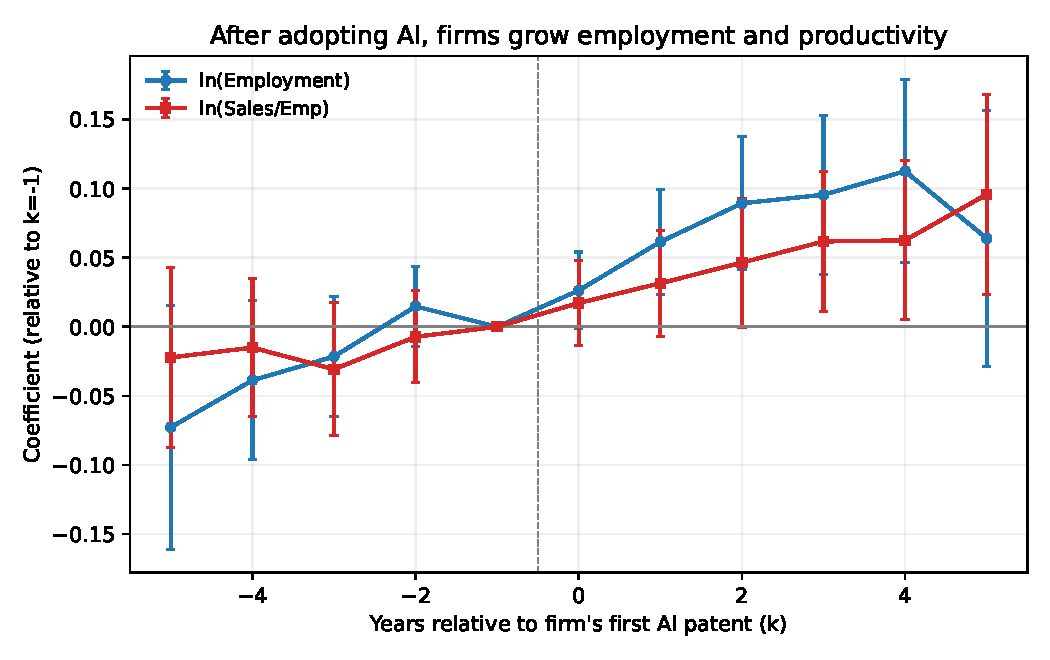
\includegraphics[width=0.8\textwidth]{fig1_ai_eventstudy.pdf}
\caption{Employment and sales-per-employee around a firm's first AI patent (event time $k$, base
$k=-1$), with firm and year fixed effects. Bands are 95\% CIs (clustered by firm). Pre-adoption
trends are flat; both outcomes rise after adoption.}\label{fig:es}
\end{figure}

\begin{figure}[htbp]\centering
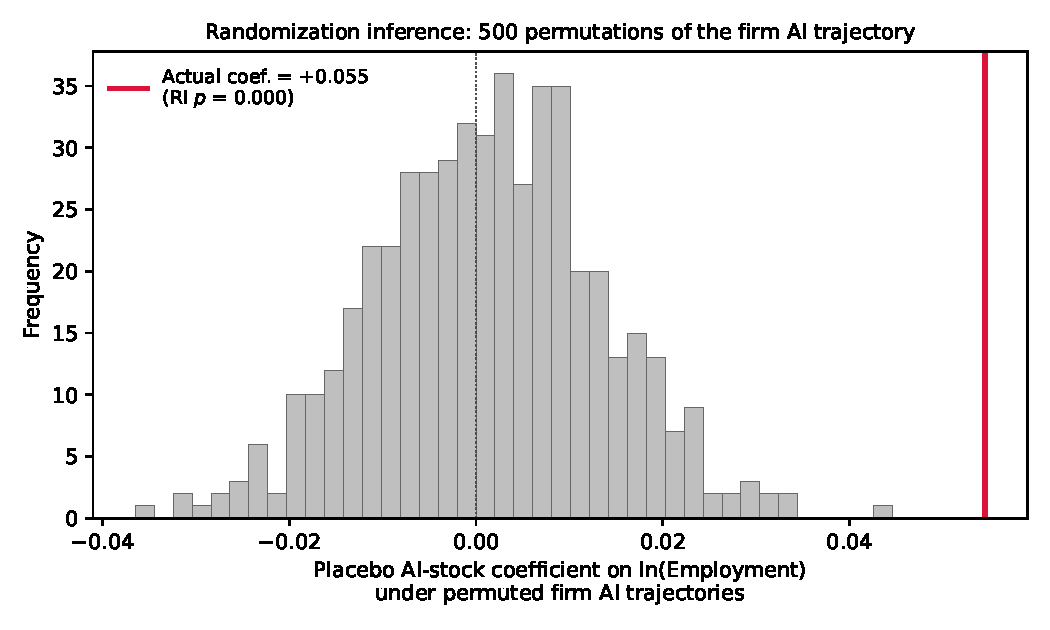
\includegraphics[width=0.72\textwidth]{fig2_randinf.pdf}
\caption{Randomization inference for the AI$\to$employment elasticity. Histogram: the distribution
of the coefficient under 500 random permutations of the firm-level AI trajectory (matched by
calendar year). The distribution is centered at zero (sharp null); the actual estimate (red line)
lies entirely outside it (RI $p<0.002$).}\label{fig:ri}
\end{figure}

\end{document}
